\documentclass[tikz,border=6pt]{standalone}
\usepackage{tikz}
\usetikzlibrary{arrows.meta,positioning}
\definecolor{nebula}{HTML}{6366F1}
\definecolor{spark}{HTML}{14B8A6}
\definecolor{ink}{HTML}{334155}
\begin{document}
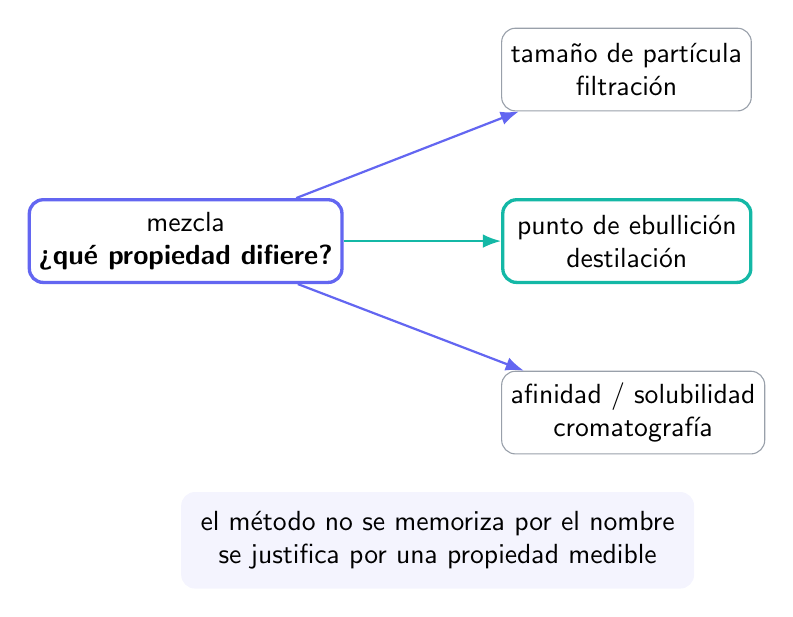
\begin{tikzpicture}[font=\sffamily,>=Latex,node distance=1.35cm,box/.style={draw=ink!50,rounded corners=5pt,minimum width=3.15cm,minimum height=1.05cm,align=center,fill=white}]
  \node[box,draw=nebula,very thick] (mix) {mezcla\\\textbf{¿qu\'e propiedad difiere?}};
  \node[box,above right=1.1cm and 2cm of mix] (size) {tama\~no de part\'icula\\filtraci\'on};
  \node[box,right=2cm of mix,draw=spark,very thick] (boil) {punto de ebullici\'on\\destilaci\'on};
  \node[box,below right=1.1cm and 2cm of mix] (affinity) {afinidad / solubilidad\\cromatograf\'ia};
  \draw[->,thick,nebula] (mix)--(size);
  \draw[->,thick,spark] (mix)--(boil);
  \draw[->,thick,nebula] (mix)--(affinity);
  \node[align=center,fill=nebula!7,rounded corners=5pt,inner sep=7pt] at (3.2,-3.8) {el m\'etodo no se memoriza por el nombre\\se justifica por una propiedad medible};
\end{tikzpicture}
\end{document}
